%
% File acl2014.tex
%
% Contact: koller@ling.uni-potsdam.de, yusuke@nii.ac.jp
%%
%% Based on the style files for ACL-2013, which were, in turn,
%% Based on the style files for ACL-2012, which were, in turn,
%% based on the style files for ACL-2011, which were, in turn, 
%% based on the style files for ACL-2010, which were, in turn, 
%% based on the style files for ACL-IJCNLP-2009, which were, in turn,
%% based on the style files for EACL-2009 and IJCNLP-2008...

%% Based on the style files for EACL 2006 by 
%%e.agirre@ehu.es or Sergi.Balari@uab.es
%% and that of ACL 08 by Joakim Nivre and Noah Smith

\documentclass[11pt]{article}
\usepackage{acl2014}
\usepackage{times}
\usepackage{url}
\usepackage{multirow}	
\usepackage{latexsym}
\usepackage{amsmath}
\usepackage{amssymb}
\usepackage{algorithm}
\usepackage{graphicx}
\usepackage[font=small,labelfont=bf]{caption}
\usepackage{subcaption}
\usepackage{enumitem}
\usepackage{bm}
\usepackage{multirow}

\usepackage{xcolor}

\DeclareMathOperator*{\argmax}{arg\,max}
\newcommand{\ts}{\textsuperscript}
\newcommand{\rione}{r^{(i)}}
\newcommand{\ritwo}{r^{(i,2)}}
\newcommand{\rithree}{r^{(i,3)}}
\newcommand{\xione}{t^{(i,1)}}
\newcommand{\xitwo}{t^{(i,2)}}
\newcommand{\xithree}{t^{(i,3)}}
\newcommand{\aione}{a_i}
\newcommand{\aitwo}{a^{(i,2)}}
\newcommand{\aithree}{a^{(i,3)}}
\newcommand{\yione}{y^{(i,1)}}
\newcommand{\yitwo}{y^{(i,2)}}
\newcommand{\yithree}{y^{(i,3)}}
\newcommand{\phii}{\phi^{(i)}}
\newcommand{\bi}{z^{(i)}}
\newcommand{\oi}{o^{(i)}}
\newcommand{\p}{{\cal P}}
\newcommand{\internal}{{\cal I}}
\newcommand{\n}{{\cal N}}
\newcommand{\rules}{{\cal R}}
\newcommand{\srule}{{X \rightarrow b, c}}
\newcommand{\pa}{\mathrm{pa}}
\newcommand{\lc}{\mathrm{lc}}
\newcommand{\rc}{\mathrm{rc}}
\newcommand{\diag}{\mathrm{diag}}
\newcommand{\tleft}{\beta}
\newcommand{\tright}{\gamma}
\newcommand{\tree}{\tau}
\newcommand{\e}[1]{\hat{#1}}
\newcommand{\commentout}[1]{}
\newcommand{\shorten}[1]{}
\newcommand{\tcommentout}[1]{#1}
\newcommand{\bS}{{\bf S}}
\newcommand{\bX}{{\bf X}}
\newfont{\msym}{msbm10}
\newcommand{\reals}{\mbox{\msym R}}
\newcommand{\qed}{{\setlength{\fboxsep}{0pt}
\framebox[7pt]{\rule{0pt}{7pt}}}}
\newcommand{\balpha}{\bm{\alpha}}
\newcommand{\bbeta}{\bm{\beta}}
\newenvironment{itemizesquish}{\begin{list}{\setcounter{enumi}{0}\labelitemi}{\setlength{\itemsep}{-0.25em}\setlength{\labelwidth}{0.5em}\setlength{\leftmargin}{\labelwidth}\addtolength{\leftmargin}{\labelsep}}}{\end{list}}
\usepackage{color}
\newcommand{\cjd}[1]{\textcolor{red}{\textbf{[#1 --CJD] }}}
\newcommand{\shaycomment}[1]{\textcolor{blue}{#1 -- Shay}}
\newcommand{\avcomment}[1]{\textcolor{orange}{\textbf{[#1 -- Av]}}}
\newcommand{\ignore}[1]{}

% You can expand the titlebox if you need extra space
% to show all the authors. Please do not make the titlebox
% smaller than 5cm (the original size); we will check this
% in the camera-ready version and ask you to change it back.
%\setlength\titlebox{5cm} %for expanding the title box
\title{Latent Variable Synchronous CFGs for Hierarchical Translation}

%\author{First Author \\
%  Affiliation / Address line 1 \\
%  Affiliation / Address line 2 \\
%  Affiliation / Address line 3 \\
%  {\tt email@domain} \\\And
%  Second Author \\
%  Affiliation / Address line 1 \\
%  Affiliation / Address line 2 \\
%  Affiliation / Address line 3 \\
%  {\tt email@domain} \\}

\date{}



\begin{document}
\maketitle
\begin{abstract}
Data-driven refinement of non-terminal categories has been demonstrated to be a reliable technique for improving monolingual parsing with PCFGs. 
In this paper, we extend these techniques to learn latent refinements of single-category synchronous grammars, so as to improve translation performance. 
We compare two estimators for this latent variable model: one based on EM and the other on the method of moments, and evaluate their performance on a Chinese--English translation task.
The results indicate that we can achieve significant gains over the baseline with both approaches, but in particular the moments-based estimator is both faster and performs better than EM.  
\end{abstract}

\section{Introduction}
Translation models based on synchronous context-free grammars (SCFGs) treat the translation problem as a context-free parsing problem. 
A parser constructs trees over the input sentence by parsing with the source language projection of a synchronous CFG, and each derivation induces translations in the target language \cite{Chiang2007}. 
However, in contrast to syntactic parsing, where linguistic intuitions can help elucidate the ``right'' tree structure for a grammatical sentence, no such intuitions are available for synchronous derivations, and so learning the ``right'' grammars is a central challenge.

\ignore{
 based on synchronous context-free grammars are state-of-the-art in many language pairs and widely studied. Most systems rely on vast inventories of translation rules about multiword phrases (e.g., French to English: \emph{un chien Andalou} $\rightarrow$ \emph{an Andalusian dog}) in addition to more minimal units (\emph{chien} $\rightarrow$ \emph{dog}). 
On top of these phrase-based approaches, the use of synchronous grammar-based formalisms \cite{Lewis1968} allows syntactic information to be explicitly incorporated in the translation process, either with category information \cite{Galley2004,SAMT,GregsTreeToStringStuff}, e.g., the French to English rule $\text{VP}\rightarrow \langle \textit{ne }\text{VB }\textit{pas}, \textit{does not }\text{VB}\rangle$ or only structural information in the form of single-category grammars \cite{Chiang2007}, e.g., the rule  $\text{X}\rightarrow \langle \textit{ne }\text{X }\textit{pas}, \textit{does not }\text{X}\rangle$.  

Single-category grammars work well in some circumstances.
Their use alleviates data sparseness issues, allows the option of building partial translations that can then be combined serially, and eliminates the need for a noisy domain-specific parser \cite{Zollmann2006}.  
However, by using only one category a significant amount of syntactic and context-specific information is discarded. 
For example, the English word \emph{plant} can translate in Spanish to both \emph{f{\'a}brica} (a factory) or \emph{plantar} (i.e., to plant a tree), depending on the part-of-speech on the English side.  
Therefore, a natural question is how we can refine synchronous grammars with learned latent categories that capture certain context-specific syntactic regularities, but without the use of hard syntactic constraints from a parser.  
}

Of course, learning synchronous grammars from parallel data is a widely studied problem \cite[\emph{inter alia}]{Wu1997,Blunsom2008,Levenberg2012}. 
However, there has been less exploration of learning rich non-terminal categories, largely because previous efforts to learn such categories have been coupled with efforts to learn derivation structures---a computationally formidable challenge.  
One popular approach has been to derive categories from source and/or target monolingual grammars \cite{Galley2004,Zollmann2006,Hanneman2013}. 
While often successful, accurate parsers are not available in many languages: a more appealing approach is therefore to learn the category structure from the data itself.

In this work, we take a slightly different approach to previous work in synchronous grammar induction by assuming that reasonable tree structures for a parallel corpus can be chosen heuristically, and then, fixing the trees (thereby enabling us to sidestep the worst of the computational issues), we learn non-terminal categories as latent variables to explain the distribution of these synchronous trees. 
This technique has a long history in monolingual parsing \cite{Petrov2006,Liang2007,cohen-14b}, where it reliably yields state-of-the-art phrase structure parsers based on generative models, but we are the first to apply it to translation.

\ignore{Our approach refines single-category (``Hiero'') synchronous grammars by incorporating additional context via a latent variable model, featurized over inside and outside sub-trees of synchronous derivation trees for source-target sentence pairs.  }
We first generalize the concept of latent PCFGs to latent variable SCFGs (\S\ref{sec:formalism}). We then follow by a presentation of the tensor-based formulation for our parameters, a representation that makes it convenient to marginalize over latent states.  
Subsequently, two methods for parameter estimation are presented (\S\ref{sec:estimation}): a spectral approach based on the method of moments, and an EM-based likelihood maximization.  
Results on a Chinese--English evaluation set (\S\ref{sec:evaluation}) indicate significant gains over baselines and point to the promise of using latent variable synchronous grammars in conjunction with a smaller, simpler set of rules instead of unwieldy and bloated grammars extracted via existing heuristics, where a large number of context-independent but un-generalizable rules are utilized.  
Hence, the hope is that this work promotes the move towards translation models that directly model the conditional likelihood of translation rules via (potentially feature-rich) latent variable models which leverage information contained in the synchronous tree structure, instead of relying on the heuristic relative frequency parameter estimates \cite{Koehn2003} from non-hierarchical phrase-based translation.  

\section{Latent Variable SCFGs}
\label{sec:formalism}

Before discussing parameter learning, we introduce latent-variable synchronous context-free grammars (L-SCFGs) and discuss an inference algorithm for marginalizing over latent states.  
%The decoder is based on simple tensor-vector products that sum over the latent states.  

We extend the definition of L-PCFGs \cite{Matsuzaki2005,Petrov2006} to synchronous grammars as used in machine translation \cite{Chiang2007}. 
%\shaycomment{is it really true? it seenms to me like our definition is for general L-SCFGs with multiple non-terminals.}
A latent variable SCFG (L-SCFG) is a 6-tuple $(\mathcal{N}, m, n_s, n_t, \pi, t)$ where: 
\begin{itemizesquish}
  \item $\mathcal{N}$ is a set of non-terminal (NT) symbols in the grammar.  
  	For HPBT, the set consists of only two symbols, \bX~and a goal symbol \bS.  
  \item $[m]$ is the set of possible hidden states associated with NTs.  
  	Aligned pairs of NTs across the source and target languages share the same hidden state.
	%In line with previous work, we assume that the states associated with NTs on the RHS are \emph{not} conditionally independent given the latent state of the left-hand side (LHS).  
   \item $[n_s]$ is the set of source side words, i.e., the source-side vocabulary, with $[n_s] \cap \mathcal{N} = \emptyset$.
   \item $[n_t]$ is the set of target side words, i.e., the target-side vocabulary, with $[n_t] \cap \mathcal{N} = \emptyset$.
   \item The synchronous production rules compose a set $\rules = \rules_0 \cup \rules_1 \cup \rules_2$:
   
$\bullet$ Binary rules ($\rules_2$): $$a(h_1) \rightarrow \langle \alpha_1b(h_2)\alpha_2c(h_3)\alpha_3, \newline \beta_1b(h_2)\beta_2c(h_3)\beta_3 \rangle$$ or $$a(h_1) \rightarrow \langle \alpha_1 b(h_2) \alpha_2 c(h_3) \alpha_3, \beta_1 c(h_2) \beta_2 b(h_3) \beta_3 \rangle$$ where $a,b,c \in \mathcal{N}$, $h_1,h_2,h_3 \in [m]$, $\alpha_1,\alpha_2,\alpha_3 \in [n_s]^{\ast}$ and $\beta_1,\beta_2,\beta_3 \in [n_t]^{\ast}$.

$\bullet$ Unary rules ($\rules_1$): $$a(h_1) \rightarrow \langle \alpha_1 b(h_2) \alpha_2, \beta_1 b(h_2) \beta_2\rangle$$ where $a,b \in \mathcal{N}$, $h_1,h_2 \in [m]$, $\alpha_1,\alpha_2 \in [n_s]^{\ast}$ and $\beta,\beta_2 \in [n_t]^{\ast}$. 

$\bullet$ Pre-terminal rules ($\rules_0$): $a(h_1) \rightarrow \langle \alpha, \beta \rangle$ where $a \in \mathcal{N}$, $\alpha \in [n_t]^{\ast}$ and $\beta \in [n_s]^{\ast}$.

Each of these rules is associated with a probability $t(a(h_1) \rightarrow \gamma | a, h_1)$ where $\gamma$ is the right-hand side (RHS) of the rule.

\ignore{
For $a =\bX, b \in [n_s] \cup \mathcal{N} \setminus \{\bS\}, c \in [n_t]
     \cup \mathcal{N} \setminus \{\bS\}, h_1, h_2, h_3 \in [m]$, we have the following context-free rules, based on the number of NT symbols \bX~in the RHS of the rule:
     \begin{itemize}
       \item Two NTs: \\
	   $a(h_1) \rightarrow ~ \langle b(h_2, h_3), c(h_2, h_3), \sim \rangle$, where $\sim$ is a one-to-one correspondence between the NT symbols of $b$ and $c$, $h_2$ is associated with one of the aligned NT pairs, and $h_3$ is associated with the other pair.  
	   The rule has an associated parameter $t(a \rightarrow b,c, h_2, h_3 | a, h_1)$
       \item One NT: \\
	   	$a(h_1) \rightarrow ~\langle b(h_2), c(h_2), \sim \rangle$, with associated parameter $t(a \rightarrow b, c, h_2 | a, h_1)$
       \item No NTs:
	   	$a(h_1) \rightarrow ~ \langle b, c,\sim \rangle$, with associated parameter $t(a \rightarrow b,c | a, h_1)$
        \end{itemize}
}
         \item For $a \in \mathcal{N}$, $h \in [m]$, $\pi(a, h)$ is a parameter specifying the root probability of $a(h)$. 
\end{itemizesquish}
%A skeletal tree (s-tree) for a sentence is a sequence of rules $r_1, \dots, r_N$ where each $r_i$ is of the form of one of the synchronous context-free rules above.\cjd{left most rewrite, relative to the source language? actually, isn't it easiest just to say it's the rules in a synchronous derivation, not decorated with latent state info?} 
A skeletal tree (s-tree) for a sentence is the set of rules in the synchronous derivation of that sentence, without any additional latent state information or decoration.  
A full tree consists of an s-tree $r_1, \dots, r_N$ together with values $h_1, \dots, h_N$ for every NT in the tree.  
An important point to keep in mind in comparison to L-PCFGs is that the right-hand side (RHS) non-terminals of synchronous rules are aligned pairs across the source and target languages.  
%In HPBT, where only rules with at most two NTs in the RHS are used, the set of rules obtained from the training corpus $\rules$ can be further divided into three non-overlapping sets $\rules_0, \rules_1, \rules_2 \in \rules$, containing the pre-terminal, unary, and binary rules respectively.   

In this work, we refine the one-category grammar introduced by \newcite{Chiang2007} for hierarchical phrase-based translation (HPBT) in order to learn additional latent NT categories.  
Thus, the following discussion is restricted to these kinds of grammars, although the method is equally applicable in other scenarios, e.g., the extended tree-to-string transducer ({\bf xRs}) formalism \cite{Huang2006,Graehl2008} commonly used in syntax-directed translation.  

\paragraph{Marginal Inference with L-SCFGs.}
\label{sec:decoding} 
\begin{figure}[h!]
	\begin{footnotesize}
	\framebox{\parbox{\columnwidth}{
		{\bf Inputs:} Sentence $f_1 \ldots f_N$, L-SCFG $(\n, S, m, n)$, parameters $C^r \in \reals^{(m \times m \times m)}$, $\in \reals^{(m \times m)}$, or $\in \reals^{(1 \times m)}$ for all $r \in \rules$, $C^\bS \in \reals^{(m \times 1)}$, hypergraph $\mathcal{H}$.  

		{\bf Data structures:} 
		
		For each node $q \in \mathcal{H}$:
		\begin{itemize}[noitemsep]
			\item $\balpha(q) \in \reals^{1 \times m}$ is a row vector of inside terms.
			\item $\bbeta(q) \in \reals^{m \times 1}$ is a column vector of outside terms.
			\item For each incoming edge $e \in {\bf B}(q)$ to node $q$, $\mu(e)$ is a marginal probability for edge (rule) $e$.			
		\end{itemize}

		{\bf Algorithm:}
		
		$\triangleright$ \emph{Inside Computation}
		%(Inside base case) $\forall i \in [N], \;\; \alpha^{X, i, i} = \sum_{r \in \bX \rightarrow f_i} C^r$
					
		For nodes $q$ in topological order in $\mathcal{H}$,
			\begin{itemize}[label={},nolistsep]
				\item $\balpha(q) = \bm{0}$
				\item For each incoming edge $e \in {\bf B}(q)$,
				\item \begin{itemize}[label={}]
						\item tail = {\bf t}(e), rule = {\bf r}(e)
						\item if $|$tail$| = 0$, then $\balpha(q) = \balpha(q) + C^{\textrm{rule}}$	
						\item else if $|$tail$| = 1$, then $\balpha(q) = \balpha(q) + C^{\textrm{rule}} \times_1 \balpha(\textrm{tail}_0)$
						\item else if $|$tail$| = 2$, then $\balpha(q) = \balpha(q) + C^{\textrm{rule}}  \times_2 \balpha(\textrm{tail}_1) \times_1 \balpha(\textrm{tail}_0)$	
					\end{itemize}
				\end{itemize}
				
				
		$\triangleright$ \emph{Outside Computation}
				
		For $q \in \mathcal{H}$,
		\begin{itemize}[label={},nolistsep]
			\item $\bbeta(q) = \bm{0}$
		\end{itemize}
		$\bbeta(\textrm{goal}) = C^\bS$
		
		For $q$ in reverse topological order in $\mathcal{H}$,
		\begin{itemize}[label={},nolistsep]
			\item For each incoming edge $e \in {\bf B}(q)$,
			\item \begin{itemize}[label={}]
				\item tail = {\bf t}(e), rule = {\bf r}(e)
				\item if $|$tail$| = 1$, then $\bbeta(\textrm{tail}_0) = \bbeta(q) \times_0 C^{\textrm{rule}}$
				\item else if $|$tail$| = 2$, then,
					\begin{itemize}[label={}]
						\item $\bbeta(\textrm{tail}_0) = \bbeta(q) \times_0 C^{\textrm{rule}} \times_2 \balpha(\textrm{tail}_1)$
						\item $\bbeta(\textrm{tail}_1) = \bbeta(q) \times_0 C^{\textrm{rule}} \times_1 \balpha(\textrm{tail}_0)$						
					\end{itemize}

			\end{itemize}
		\end{itemize}
			

		\hbox{$\triangleright$\emph{Edge Marginals}}
		Sentence probability $g = \balpha(\textrm{goal}) \times \bbeta(\textrm{goal})$
		
		For edge $e \in \mathcal{H}$, 
			\begin{itemize}[label={},nolistsep]
					\item head = {\bf h}(e), tail = {\bf t}(e), rule = {\bf r}(e)
					\item if $|$tail$| = 0$, then $\mu(e) = (\bbeta(\textrm{head}) \times_0 C^{\textrm{rule}}) / g$
					\item else if $|$tail$| = 1$, then $\mu(e) = (\bbeta(\textrm{head}) \times_0 C^{\textrm{rule}} \times_1 \balpha(\textrm{tail}_0)) / g$
					\item else if $|$tail$| = 2$, then $\mu(e) = (\bbeta(\textrm{head}) \times_0 C^{\textrm{rule}} \times_2 \balpha(\textrm{tail}_1) \times_1 \balpha(\textrm{tail}_0)) / g$					
			\end{itemize}
}}
\end{footnotesize}
\caption{The tensor form of the hypergraph inside-outside algorithm, for calculation of rule marginals $\mu(e)$.  
A slight simplification in the marginal computation yields NT marginals for spans $\mu(\bX, i, j)$.
{\bf B}(q) returns the incoming hyperedges for node $q$, and {\bf h}(e), {\bf t}(e), {\bf r}(e) return the head node, tail nodes, and rule for hyperedge $e$.} 
\vspace{-0.5cm}
\label{fig:hg_io_spec}
\end{figure}
For a parameter $t$ of rule $r$, the latent state $h_1$ attached to the left-hand side (LHS) NT of $r$ is associated with the outside tree for the sub-tree rooted at the LHS, and the states attached to the RHS NTs are associated with the inside trees of that NT.    
Since we do not assume conditional independence of these states, we need to consider all possible interactions, which can be compactly represented as a 3\ts{rd}-order tensor in the case of a binary rule, a matrix (i.e., a 2\ts{nd}-order tensor) for unary rules, and a vector for pre-terminal (lexical) rules.  
Preferences for certain outside-inside tree combinations are reflected in the values contained in these tensor structures.  
In this manner, we intend to capture interactions between non-local context, as represented by the outside tree, and local context, through the inside trees. 
We refer to these tensor structures collectively as $C^r$ for rules $r \in \rules$, which encompass the parameters $t$.  

For $r \in \rules_0: C^r \in \reals^{1 \times m}$; similarly for $r \in \rules_1: C^r \in \reals^{m \times m}$ and $r \in \rules_2: C^r \in \reals^{m \times m \times m}$.
We also maintain a vector $C^\bS \in \reals^{m \times 1}$ corresponding to the parameters $\pi(\bS, h)$ for the goal node (root).   
These parameters participate in tensor-vector operations: a 3\ts{rd}-order tensor $C^{r_2}$ can be multiplied along each of its three modes ($\times_0, \times_1, \times_2$), and if multiplied by an $m \times 1$ vector, will produce an $m \times m$ matrix.\footnote{This operation is sometimes called a contraction.}
Note that matrix multiplication can be represented by $\times_1$ when multiplying on the right and $\times_0$ when multiplying on the left of the matrix.  

The decoder computes probabilities for each rule in the parse forest of a source sentence by marginalizing over the latent states, which in practice corresponds to simple tensor-vector products, and is not dependent on the manner in which the parameters were estimated. 
Figure \ref{fig:hg_io_spec} presents the tensor version of the inside-outside algorithm for decoding L-SCFGs. 
The algorithm takes as input the parse forest of the source sentence represented as a hypergraph \cite{Klein2001}, which is computed using a bottom-up parser with Earley-style rules similar to the algorithm in \newcite{Chiang2007}.  
Then, the algorithm computes inside and outside probabilities over the hypergraph using the tensor representations, and converts these probabilities to marginal rule probabilities.  
It is similar to the version presented in \newcite{cohen-14b}, but adapted to hypergraph parse forests. 
 
The complexity of this decoding algorithm is $\mathcal{O}(n^3 m^3 |G|)$ where $n$ is the length of the input sentence, $|G|$ is the number of production rules in the grammar \emph{without} latent-variable annotations (i.e., $1$ in this paper), and $m$ is the number of latent states.
The bulk of the computation is a series of tensor-vector products of relatively small size (each dimension is of length $m$), which can be computed very quickly and in parallel.
%The algorithm maintains its $\mathcal{O}(n^3|G|)$ complexity where $n$ is the length of the input sentence and $|G|$ is the size of the grammar; \shaycomment{what do you mean by the following? increase the number of rules compared to what? the grammar size is the same as what?} we do not increase the number of rules at all, so the grammar size is the same. 
%But of course, there is no free lunch, and the additional computation gets shifted to the marginalization over latent states via the algorithm in Figure \ref{fig:hg_io_spec}.  
%The bulk of the computation is a series of tensor-vector products of relatively small size (each dimension is of length $m$), which can be computed very quickly and in parallel.
%\shaycomment{are we really parallelizing the decoding, or you are just suggesting that it is somehow possible? what can be done in a parallel manner?}
%\avcomment{we really are parallelizing the decoding, but I'm parallelizing at the level of sentences.  What I meant here is that each tensor-vector dot product can be parallelized in that the dot product along each dimension can be computed at the same time, which is how most matrix multiplication packages work right?} 
%In addition, 
The tensor computations can be significantly sped up using techniques described by \newcite{cohen-12c}, so that they are linear in $m$ and not cubic.  



\section{Derivation Trees for Parallel Sentences}
\label{sec:mingrammar}
To estimate the parameters $t$ and $\pi$ of an L-SCFG (discussed in detail in the next section), we assume the existence of a dataset composed of synchronous s-trees, which can be acquired from word alignments.  
Normally in phrase-based translation models, we consider all possible phrase pairs consistent with the word alignments and estimate features based on surface statistics associated with the phrase pairs or rules. 
The weights of these features are then learned using some kind of discriminative training algorithm \cite{Och2003,Chiang2012}.  
%a dataset composed of synchronous s-trees is required.\cjd{not required, but we assume we have it for simplicity's sake. we need to make clear what our assumptions are up front because this is quite different from how parameters are usually learned in translation models}
In contrast, in this work we restrict the number of possible synchronous derivations for each sentence pair to just one; thus, derivation forests do not have to be considered, making parameter estimation more tractable.  

To achieve this objective, for each sentence in the training data we extract the {\bf minimal} set of synchronous rules consistent with the word alignments, as opposed to the {\bf composed} set of rules.  
Composed rules are ones that can be formed out of smaller rules in the grammar; with these rules, there are multiple synchronous trees consistent with the alignments for a given sentence pair, and thus the total number of applicable rules can be combinatorially larger than if we just consider the set of rules that cannot be formed from other rules, namely the minimal rules.  
The rule types across all sentence pairs are combined to form a minimal grammar.\footnote{In our experiments (\S\ref{sec:data}), a grammar extracted using the traditional Hiero heuristics was more than 80 times larger than the minimal grammar.} 

%\shaycomment{
%I want to rephrase your text below, because it does not make it clear that we are using minimal rules.
%I am confused about the process though, is it that the Gildea algorithm extracts a minimal grammar or synchronous s-trees?
%Can you also roughly describe how the algorithm works in a few key sentences?}
%In order to learn the parameters $t$, we need a set of synchronous s-trees, which can be acquired from word alignments.  
%For each rule $r_i$ in each s-tree, we can either compute partial counts in the expectation step of the EM algorithm, or extract second-order moments of features on which we compute an SVD.  
%During the extraction phase, if we consider {\bf composed} rules, namely rules that can be formed out of smaller rules in the grammar, then there are multiple synchronous trees consistent with the alignments for a given sentence pair, and thus the total number of applicable rules can be combinatorially larger than if we just consider the set of {\bf minimal} rules i.e., rules that cannot be formed from other rules. 
To extract a set of minimal rules for each word-aligned sentence pair, we use the linear-time extraction algorithm of \newcite{Zhang2008}.  
This algorithm generalizes an approach for finding all common intervals (a pair of phrases such that no word pair in the alignment links a word inside the phrase to a word outside the phrase) between two permutations to sequences with many-to-many alignment links between the two sides, as in word alignment. 
%\avcomment{Should we talk about how rules with $>$ 2 NTs in the RHS are generated, and how we handle?}
By using minimal rules as a starting point instead of the traditional heuristically-extracted rules \cite{Chiang2007} or arbitrary compositions of minimal rules \cite{Galley2006}, we are also able to explore the transition from minimal rules to composed ones in a principled manner by encoding contextual information through the latent states.   
Thus, a beneficial side effect of our refinement process is the creation of more context-specific rules without increasing the overall size of the grammar.

\section{Parameter Estimation for L-SCFGs}
\label{sec:estimation}
We explore two methods for estimating the parameters $C^r$ of the model: a likelihood-maximization approach based on EM \cite{Dempster1977}, and a spectral approach based on the method of moments \cite{Hsu2009,cohen-14b}, where we identify a subspace using a singular value decomposition (SVD) of the cross-product feature space between inside and outside trees and estimate parameters in this subspace. 
%\cite{Golub1996}

Figure \ref{fig:estimation-algos} presents a side-by-side comparison of the two algorithms, which we discuss in this section.  
In the spectral approach, we base our parameter estimates on low-rank representations of moments of features, while EM explicitly maximizes a likelihood criterion. 
The parameter estimation algorithms are relatively similar, but in lieu of sparse feature functions in the spectral case, EM uses partial counts estimated with the current set of parameters.  
The nature of EM allows it to be susceptible to local optima, while the spectral approach comes with guarantees on obtaining the global optimum. 
Lastly, computing the SVD and estimating parameters in the low-rank space is a one-shot operation, as opposed to the iterative procedure of EM. 

\begin{figure*}[t!]
	\centering
	\fbox{
	\begin{footnotesize}		
	\begin{subfigure}{0.87\columnwidth}
	{\bf Inputs:} 
	
	Training examples $(\rione, \xione, \xitwo, \xithree, \oi, b^{(i)})$ for $i \in \{1 \ldots M\}$, where $\rione$ is a context free rule; $\xione$, $\xitwo$, and $\xithree$ are inside trees; $\oi$ is an outside tree; and $b^{(i)} = 1$ if the rule is at the root of tree, $0$ otherwise.
A function $\phi$ that maps inside trees $t$ to feature-vectors $\phi(t) \in \reals^d$. A function $\psi$ that maps outside trees $o$ to feature-vectors $\psi(o) \in \reals^{d'}$.

	{\bf Algorithm:}
	%If $\rione$ is of the form $\srule$, define $b_i$ to be the non-terminal for the left-child of $\rione$, and $c_i$ to be the non-terminal for the right-child.

	$\triangleright$ \emph{Step 0: Singular Value Decomposition}
	\begin{itemize}
		\item Compute the SVD of Eq.~\ref{eq:outerproduct} to calculate matrices $\e{U} \in \reals^{(d \times m)}$ and $\e{V} \in \reals^{(d' \times m)}$.
	\end{itemize}

	$\triangleright$ \emph{Step 1: Projection}
	\begin{align*}
		Y(t) &= U^{\top} \phi(t)\\
		Z(o) &= \Sigma^{-1} V^{\top} \psi(o)
	\end{align*}

	$\triangleright$ \emph{Step 2: Calculate Correlations}
	\begin{align*}
		\e{E}^r &= \begin{cases}
			\frac{\sum_{o \in Q^r} Z(o)}{|Q^r|} &  \textrm{if }r \in \rules_0 \\
			\frac{\sum_{\left(o, t\right) \in Q^r} Z(o) \otimes Y(t)}{|Q^r|} & \textrm{if }r \in \rules_1 \\
			\frac{\sum_{\left(o, t^2, t^3\right) \in Q^r} Z(o) \otimes Y(t^2) \otimes Y(t^3)}{|Q^r|} & \textrm{if }r \in \rules_2 
		\end{cases}
	\end{align*}
	$Q^r$ is the set of outside-inside tree triples for binary rules, outside-inside tree pairs for unary rules, and outside trees for pre-terminals.

	$\triangleright$ \emph{Step 3: Compute Final Parameters}
	\begin{itemize}
		\item For all $r \in \rules$, 
			\begin{itemize}[label={}]
				\item $\e{C}^r = \frac{\textrm{count}(r)}{M} \times \e{E}^r$
			\end{itemize}
		\item For all $\rione \in \{1, \dots, M\}$ such that $b^{(i)}$ is 1, 
		\begin{itemize}[label={}]
			\item $\e{C}^\bS =  \e{C}^\bS + \frac{Y(\xione)}{|Q^\bS|} $
		\end{itemize}						
	\end{itemize}
	$Q^\bS$ is the set of trees at the root.  

$\,$

$\,$

$\,$

$\,$

$\,$

$\,$

$\,$

$\,$

$\,$

$\,$
	\caption{\small The spectral learning algorithm for estimating parameters of an L-SCFG.}
	\label{fig:splearn}
	\end{subfigure}
	%&
	\begin{subfigure}{1.05\columnwidth}
	{\bf Inputs:} 
	
	Training examples $(\rione, \xione, \xitwo, \xithree, \oi, b^{(i)})$ for $i \in \{1 \ldots M\}$, where $\rione$ is a context free rule; $\xione$, $\xitwo$, and $\xithree$ are inside trees; $\oi$ is an outside tree; $b^{(i)} = 1$ if the rule is at the root of tree, $0$ otherwise; and MAX\_ITERATIONS.
%A function $\phi$ that maps inside trees $t$ to feature-vectors $\phi(t) \in \reals^d$. A function $\psi$ that maps outside trees $o$ to feature-vectors $\psi(o) \in \reals^{d'}$.

	{\bf Algorithm:}
	%If $\rione$ is of the form $\srule$, define $b_i$ to be the non-terminal for the left-child of $\rione$, and $c_i$ to be the non-terminal for the right-child.

	$\triangleright$ \emph{Step 0: Parameter Initialization}
	
	For rule $r \in \rules$,
	\begin{itemize}[noitemsep]
		\item if $r \in \rules_0$: initialize $\e{C}^r \in \reals^{1 \times m}$ 
		\item if $r \in \rules_1$: initialize $\e{C}^r \reals^{m \times m}$ 
		\item if $r \in \rules_2$: initialize $\e{C}^r \reals^{m \times m \times m}$ 
	\end{itemize}
	
	Initialize $\e{C}^\bS \in \reals^{m \times 1}$ 
	
	$\e{C}_0^r = \e{C}^r, \e{C}_0^\bS = \e{C}^\bS$
	
	For iteration $t=1, \dots, \textrm{MAX\_ITERATIONS}$, 
	\begin{itemize}			
		\item Expectation Step: 
		 \begin{itemize}[label={}]
			\item $\triangleright$ \emph{Estimate $Y$ and $Z$}
			
			Compute partial counts and total tree probabilities $g$ for all $t$ and $o$ using Fig.~\ref{fig:hg_io_spec} and parameters $\e{C}_{t-1}^r, \e{C}_{t-1}^\bS$.  
			\item $\triangleright$ \emph{Calculate Correlations}
				\begin{align*}
					\e{E}^r &= \begin{cases}
					\sum\limits_{o, g \in Q^r} \frac{Z(o)}{g} &\textrm{if }r \in \rules_0 \\
					\sum\limits_{\left(o, t, g\right) \in Q^r} \frac{Z(o) \otimes Y(t)}{g} &\textrm{if }r \in \rules_1 \\
					\sum\limits_{\left(o,t^2,t^3,g\right) \in Q^r} \frac{Z(o) \otimes Y(t^2) \otimes Y(t^3)}{g} &\textrm{if }r \in \rules_2 
					\end{cases}
				\end{align*}
			\item $\triangleright$ \emph{Update Parameters}
		 	\begin{itemize}[label={}]
		 		\item For all $r \in \rules$, $\e{C}^r_t = \e{C}^r_{t-1} \odot \e{E}^r$
		 		\item For all $\rione \in \{1, \dots, M\}$ such that $b^{(i)}$ is 1, $\e{C}^\bS_t = \e{C}^\bS_t + (\e{C}^\bS_{t-1} \odot Y(\rione)) / g $
		 	\end{itemize}
		 	$Q^\bS$ is the set of trees at the root.
		\end{itemize}
		\item Maximization Step
			\begin{itemize}[label={},nolistsep]%[nolistsep]
				\item if $r \in \rules_0$: $\forall h_1: \e{C}^r(h_1) = \frac{\e{C}^r(h_1)}{\sum_{r'=r} \sum_{h_1}\e{C}^{r'}(h_1)}$ 
				\item if $r \in \rules_1$: $\forall h_1, h_2: \e{C}^r(h_1, h_2) = \frac{\e{C}^r(h_1, h_2)}{\sum_{r'=r} \sum_{h_2}\e{C}^{r'}(h_1, h_2)}$ 
				\item if $r \in \rules_2$: $\forall h_1, h_2, h_3: \e{C}^r(h_1, h_2, h_3) = \frac{\e{C}^r(h_1, h_2, h_3)}{\sum_{r'=r}\sum_{h_2, h_3}\e{C}^{r'}(h_1, h_2, h_3)}$ 
				\item if $\textrm{LHS}(r) = \bS$: $\forall h_1: \e{C}^r(h_1) = \frac{\e{C}^r(h_1)}{\sum_{r'=r} \sum_{h_1}\e{C}^{r'}(h_1)}$ 
				%NEED TO MENTION NORMALIZATION FOR PI PARAMETERS
			\end{itemize}
	\end{itemize}		
	\caption{\small The EM-based algorithm for estimating parameters of an L-SCFG.}
	\label{fig:emlearn}	
	\end{subfigure}		
	\end{footnotesize}}
	\caption{The two parameter estimation algorithms proposed for L-SCFGs; (\textbf{a}) method of moments; (\textbf{b}) expectation maximization. $\odot$ is the element-wise multiplication operator.
	%\cjd{possible to get a vertical line?}
	}
	\vspace{-0.2cm}
	\label{fig:estimation-algos}
\end{figure*}

\subsection{Estimation with Spectral Method}
\label{sec:spectral} 
We generalize the parameter estimation algorithm presented in \newcite{Cohen2013} to the synchronous or bilingual case. 
The central concept of the spectral parameter estimation algorithm is to learn an $m$-dimensional representation of inside and outside trees by defining these trees in terms of features, in combination with a projection step (SVD), with the hope being that the lower-dimensional space captures the syntactic and semantic regularities among rules from the sparse feature space. 
%The spectral method relies on computing the empirical covariances between two feature spaces, represented by their respective feature functions that map tree fragments to feature vectors.  
Every NT in an s-tree has an associated inside and outside tree; the inside tree contains the entire sub-tree at and below the NT, and the outside tree is everything else in the synchronous s-tree except the inside tree.   
The inside feature function $\phi \in \mathbb{R}^d$ maps the domain of inside tree fragments to a $d$-dimensional Euclidean space, and the outside feature function $\psi \in \mathbb{R}^{d'}$ maps the domain of outside tree fragments to a $d'$-dimensional space. 
The specific features we used are discussed in \S\ref{sec:features}.  

Let $\mathcal{O}$ be the set of all tuples of inside-outside trees in our training corpus, whose size is equivalent to the number of rule tokens $M$, and let $\phi(t) \in \reals^{d \times 1}$, $\psi(o) \in \reals^{d' \times 1}$ be the inside and outside feature functions. 
By computing the outer product $\otimes$ between the inside and outside feature vectors for each pair and aggregating, we obtain the empirical inside-outside feature covariance matrix:
\begin{align}
	\hat{\Omega} = \frac{1}{|\mathcal{O}|} \sum_{(o,t) \in \mathcal{O}} \phi(t) \left(\psi(o)\right)^{\top}
	\label{eq:outerproduct}
\end{align}
If $m$ is the desired latent space dimension, we compute an $m$-rank truncated SVD of the empirical covariance matrix $\hat{\Omega} = U \Sigma V^{\top}$, where $U \in \mathbb{R}^{d \times m}$ and $V \in \mathbb{R}^{d' \times m}$ are the matrices containing the left and right singular vectors, and $\Sigma \in \mathbb{R}^{d \times d'}$ is a diagonal matrix containing the $m$-largest singular values along its diagonal.  

Figure \ref{fig:splearn} provides the remaining steps in the algorithm.  
In step 1, for each inside and outside tree, we project its high-dimensional representation to the latent space.  
Using the lower-dimensional representations for inside and outside trees, in step 2 for each rule type $r$ we compute the covariance between the inside tree vectors and the outside tree vector using the \emph{tensor product}, a generalized outer product to compute covariances between more than two random vectors.  
For binary rules, with two child inside vectors and one outside vector, the result $\e{E}^r$ is a 3-mode tensor; for unary rules, a regular matrix, and for pre-terminal rules with no right-hand side non-terminals, a vector. 
The final parameter estimate is then the associated tensor/matrix/vector, scaled by the maximum likelihood estimate of the rule $r$, as in step 3.  

The corresponding theoretical guarantees from \newcite{cohen-14b} can also be generalized to the synchronous case.  
$\hat{\Omega}$ is an empirical estimate of the true covariance matrix $\Omega$, and if $\Omega$ has rank $m$, then the marginals computed using the spectrally-estimated parameters will converge to the true marginals.  
The sample complexity for convergence is inversely proportional to the $m^{\textrm{th}}$ largest singular value.   

\subsection{Estimation with EM}
\label{sec:em}
A likelihood maximization approach can also be used to learn the parameters of an L-SCFG.  
Parameters are initialized by sampling each parameter value $\e{C}^r(h_1, h_2, h_3)$ from the interval $[0,1]$ uniformly at random.\footnote{In our experiments, we also tried the initialization scheme described in \newcite{Matsuzaki2005}, but found that it provided little benefit.}
We first decode the training corpus using an existing set of parameters to compute the inside and outside probability vectors associated with NTs for every rule in each s-tree, constrained to the tree structure of the training example. 
These probabilities can be computed using the decoding algorithm in Figure \ref{fig:hg_io_spec} (where $\balpha$ and $\bbeta$ correspond to the inside and outside probabilities respectively), except the parse forest consists of a single tree only. 
Each of these vectors represents partial counts over latent states.  
We can then define functions $Y$ and $Z$ (analogous to the spectral case) which map inside and outside tree instances to $m$-dimensional vectors containing these partial counts. 
In the spectral case, $Y$ and $Z$ are estimated just once, while in the case of EM they have to be re-estimated at each iteration.

The expectation step thus consists of computing the partial counts of inside and outside trees $t$ and $o$, i.e., recovering the functions $Y$ and $Z$, and updating parameters $C^r$ by computing correlations, which involves summing over partial counts (across all occurrences of a rule in the corpus). 
Each partial count's contribution is divided by a normalization factor $g$, which is the total probability of the tree which $t$ or $o$ is part of.  
Note that unlike the spectral case, there is a specific normalization factor for each inside-outside tuple. 
Lastly, the correlations are scaled by the existing parameter estimates.

To obtain the next set of parameters, in the maximization step we normalize $\e{C}^r$ for $r \in \rules$ such that for every $h_1, \sum_{r'=r,h_2,h_3} \e{C}^{r'}(h_1, h_2, h_3) = 1$ for $r \in \rules_2$, $\sum_{r'=r,h_2} \e{C}^{r'}(h_1, h_2) = 1$ for $r \in \rules_1$, and $\sum_{r'=r,h_2} \e{C}^{r'}(h_2) = 1$ for $r \in \rules_0$.  
We also normalize the root rule parameters $\e{C}^r$ where LHS$(r) = \bS$.  
It is also possible to add sparse, overlapping features to an EM-based estimation procedure \cite{Berg-Kirkpatrick2010} and leave this for future work.  

\section{Experiments}
\label{sec:evaluation}
%\shaycomment{what is the goal of the experiments? can you also state in the beginning the main conclusions you get out of the experiments? (preferably in a concise bulleted list.)}
The goal of the experimental section is to evaluate the performance of the latent variable SCFG in comparison to a baseline without any additional NT annotations (\textsc{Min-Grammar}), and to compare the performance of the two parameter estimation algorithms.
We also compare L-SCFGs to a \textsc{Hiero} baseline \cite{Chiang2007}. 
The language pair of evaluation is Chinese--English (\textsc{ZH-EN}).  

We score translations using BLEU \cite{Papineni2002}.  
The latent variable model is integrated into the standard MT pipeline by computing marginal probabilities for each rule in the parse forest of a source sentence using the algorithm in Figure \ref{fig:hg_io_spec} with the parameters estimated through the algorithms in Figure \ref{fig:estimation-algos}, and is added as a feature for the rule during MERT \cite{Och2003}.  
These probabilities are conditioned on the LHS (\bX), and are thus joint probabilities for a source-target RHS pair.  
We also write out as features the conditional probabilities $P(e|f)$ and $P(f|e)$ as estimated by our latent variable model, i.e., conditioned on the source and target RHS.  

Overall, we find that both the spectral and the EM-based estimators improve upon a minimal grammar baseline with only a single category, but the spectral approach does better. 
In fact, it matches the performance of the standard \textsc{Hiero} baseline, despite learning on top of a minimal grammar.  

\subsection{Data and Baselines}
\label{sec:data}
%The \textsc{DE-EN} parallel corpus is taken from the news commentary section of the WMT 2012 translation evaluation; \textsc{news-test2010} is used as the development set, and \textsc{news-test2011} is the test set.\footnote{http://www.statmt.org/wmt12/}
%The development and test sets are evaluated with a single reference.    
The \textsc{ZH-EN} data is the BTEC parallel corpus \cite{Paul2009}; we combine the first and second development sets in one, and evaluate on the third development set.   
The development and test sets are evaluated with 16 references.  
Statistics for the data are shown in Table \ref{tab:corpusstats}.  
We used the \textsc{cdec} decoder \cite{Dyer2010} to extract word alignments and the baseline hierarchical grammars, for MERT tuning, and decoding.  
We used a 4-gram language model built from the target-side of the parallel training data. 
The Python-based implementation of the tensor-based decoder, as well as the parameter estimation algorithms is available at \texttt{www.github.com/X}.  
\begin{table}[h!]
%{\small
  \begin{center}
    \begin{tabular}{p{0.5\linewidth}r}
      \hline
      & \textsc{ZH-EN} \\
	  \hline
      TRAIN (SRC)  & 334K \\
	  TRAIN (TGT)  &  366K \\
	  DEV (SRC)  & 7K \\
      DEV (TGT)  &  7.6K\\
	  TEST (SRC)  &  3.8K \\
	  TEST (TGT)  & 3.9K \\
	\end{tabular}
  \end{center}
  \caption{Corpus statistics (in words).  For the target DEV and TEST statistics, we take the first reference.}
  \label{tab:corpusstats}
  %}
\end{table}

The baseline \textsc{hiero} system uses a grammar extracted by applying the commonly used heuristics \cite{Chiang2007}.  
Each rule is decorated with two lexical and phrasal features corresponding to the forward $P(e|f)$ and backward $P(f|e)$ probabilities, along with the joint probability $P(e,f)$, the marginal probability of the source phrase $P(f)$, and whether the phrase pair or the source phrase is a singleton. 
Weights for the language model (and language model OOV), glue rule, and word penalty are also tuned. 
The \textsc{Min-Grammar} baseline maintains the same set of weights. 

\subsection{Spectral Features}
\label{sec:features}
We use the following set of sparse, binary features in the spectral learning process:
\begin{itemizesquish}
	\item \textbf{Rule Indicator.} For the inside features, we consider the rule production containing the current non-terminal on the left-hand side, as well as the rules of the children (distinguishing between left and right children for binary rules).  
	For the outside features, we consider the parent rule production along with the rule production of the sibling (if it exists). 
	\item \textbf{Lexical.} for both the inside and outside features, any lexical items that appear in the rule productions are recorded.  
	Furthermore, we consider the first and last words of spans (left and right child spans for inside features, distinguishing between the two if both exist, and sibling span for outside features).  
	Source and target words are treated separately. 
	%\item Arity: the number of non-terminals present in inside tree and outside tree rules.  
	\item \textbf{Length.} the span length of the tree and each of its children for inside features, and the span length of the parent and sibling for outside features. 	
\end{itemizesquish}
In our experiments, we used a total of 170,000 rule indicator features, 155,000 lexical features, and 80 length features.  

\subsection{Chinese--English Experiments}
Table \ref{tab:zh-en-results} presents a comprehensive evaluation of the \textsc{ZH-EN} experimental setup.  
The first section consists of the various baselines we consider. 
In addition to the aforementioned baselines, we evaluated a setup where the spectral parameters simply consist of the joint maximum likelihood estimates of the rules.  
This baseline should perform \emph{en par} with \textsc{Min-Grammar}, which we see is the case on the development set.  
The performance on the test set is better though, primarily because we also include the reverse probability $P(f|e)$ computed from the latent variable model as an additional feature in MERT.  
Furthermore, in line with previous work \cite{Galley2006} which compares minimal and composed rules, we find that minimal grammars take a hit of more than 2.5 BLEU points on the development set, compared to composed (\textsc{hiero}) grammars.  
The $m=1$ spectral baseline with only rule indicator features performs slightly better than the minimal grammar baseline, since it overtly takes into account inside-outside tree combination preferences in the parameters, but improvement is minimal with one latent state naturally and the performance on the test set is in line with the MLE baseline.  

\begin{table}[t!]
\begin{small}
  \begin{center}
    \begin{tabular}{|l|p{0.45\columnwidth}rr|}
      \hline
	  & & \multicolumn{2}{c|}{\bf BLEU} \\
      & Setup & Dev & Test \\
	  \hline
	  \multirow{3}{*}{Baselines} & \textsc{hiero} & 46.08 & 55.31 \\
      & Minimal Grammar & 43.38 & 51.78 \\
	  & MLE & 43.24 & 52.80 \\ \hline
	  \multirow{4}{*}{Spectral} &  $m=1$ RI & 44.18 & 52.62 \\
	  & $m=8$ RI & 44.60 & 53.63 \\
	  & $m=16$ RI & 46.06 & 55.83 \\
	  & $m=16$ RI+Lex+Sm & 46.08 & 55.22 \\ 
	  & $m=16$ RI+Lex+Len & 45.70 & 55.29 \\ 
	  & $m=24$ RI+Lex & 43.00 & 51.28 \\ 
	  & $m=32$ RI+Lex & 43.06 & 52.16 \\ \hline
	  \multirow{2}{*}{EM} & $m=8$ 40 iterations & 40.67 & 49.11 \\
	  & $m=16$ 30 iterations & 42.69 & 52.91 \\
	  & $m=32$ 35  iterations & 40.85 & 50.34 \\
	  \hline
	\end{tabular}
  \end{center}
  \caption{Results for the \textsc{ZH-EN} corpus, comparing across the baselines and the two parameter estimation techniques.
  RI, Lex, and Len correspond to the rule indicator, lexical, and length features respectively, and Sm denotes smoothing.
  For the EM experiments, we selected the best scoring iteration by tuning weights for parameters obtained after 25 iterations and evaluating other parameters with these weights. }
  \label{tab:zh-en-results}
\end{small}
\end{table}

On top of the baselines, we looked at a number of feature combinations and latent states for the spectral and EM-estimated latent variable models.  
For the spectral models, we tuned MERT parameters separately for each rank on a set of parameters estimated from rule indicator features only; subsequent variations within a given rank, e.g., the addition of lexical or length features or smoothing, were evaluated with the same set of rank-specific weights from MERT. 
For EM, we ran parameter estimation for 50 iterations, and tuned the MERT parameters after 25 iterations. 
Similar to the spectral experiments, we fixed the MERT weight values and evaluated BLEU performance with parameters after every 5 iterations and chose the iteration with the highest score on the development set. 

Firstly, we can see a clear dependence on rank, with peak performance for the spectral and EM models occurring at $m=16$. 
In this instance, the spectral model roughly matches the performance of the \textsc{hiero} baseline, but it only uses rules extracted from a minimal grammar, whose size is a fraction of the \textsc{hiero} grammar.  
The gains seem to level off at this rank; additional ranks seem to add noise to the parameters. 
Feature-wise, additional lexical and length features add little, probably because much of this information is encapsulated in the rule indicator features. 
For EM, $m=16$ outperforms the minimal grammar baseline, but is not at the level of the spectral results.  

The two estimation algorithms differ significantly in their estimation time.  
The spectral algorithm is one or two orders magnitude faster: it completes the entire estimation process in the same time that EM takes for one or two iterations. 

\ignore{
\subsection{\textsc{DE-EN} Experiments}
Table \ref{tab:de-en-results} presents a comprehensive evaluation of the \textsc{DE-EN} experimental setup.  
\begin{table}[t!]
\begin{small}
  \begin{center}
    \begin{tabular}{|l|p{0.45\columnwidth}rr|}
      \hline
	  & & \multicolumn{2}{c|}{\bf BLEU} \\
      & Setup & Dev & Test \\
	  \hline
	  \multirow{3}{*}{Baselines} & \textsc{hiero} & 18.50 & 16.89 \\
      & Minimal Grammar & 17.01 & 15.42 \\
	  & MLE & X & Y \\ \hline
	  \multirow{4}{*}{Spectral} &  $m=1$ RI & 17.09 & 15.34 \\
	  & $m=1$ RI+Lex+Len & X & Y \\
	  & $m=16$ RI+Lex+Len & X & Y \\
	  & $m=16$ RI+Lex+Len+Sm & X & Y \\ \hline
	  \multirow{2}{*}{EM} & $m=1$ 100 Iter & X & Y \\
	  & $m=16$ 100 Iter & X & Y \\
	  \hline
	\end{tabular}
  \end{center}
  \caption{Results for the \textsc{DE-EN} corpus, comparing across the baselines and the two parameter estimation techniques.
  RI, Lex, and Len correspond to the rule indicator, lexical, and length features respectively, and Sm denotes smoothing.}
  \label{tab:de-en-results}
\end{small}
\end{table}}

\subsection{Discussion \& Analysis}
\begin{figure*}[t!]
	\begin{center}
	\begin{subfigure}{0.67\columnwidth}
		\centering
		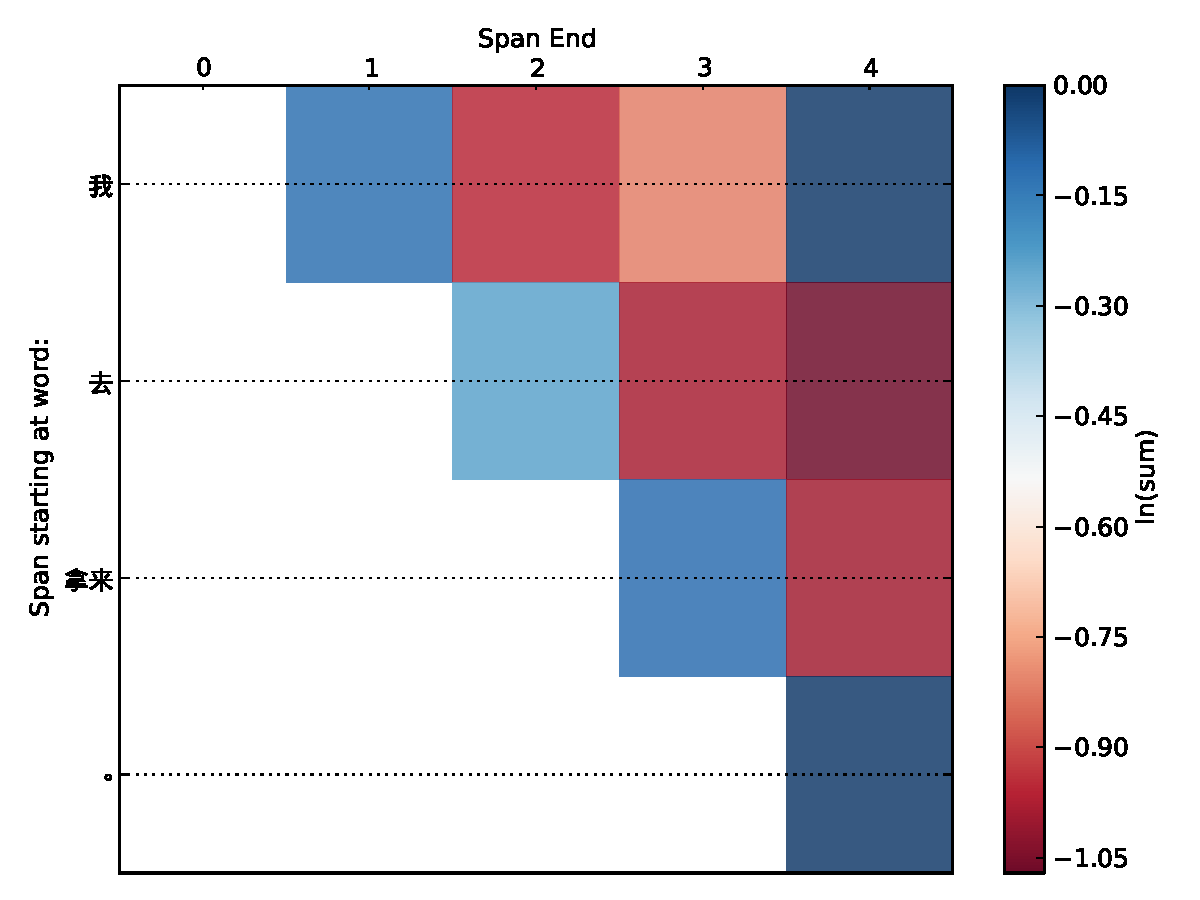
\includegraphics[width=1.1\columnwidth,keepaspectratio=true]{./mle0.pdf}	
		I go away .
		\caption{\small MLE}
		\label{fig:mle0}			
	\end{subfigure}
	\begin{subfigure}{0.67\columnwidth}
		\centering
		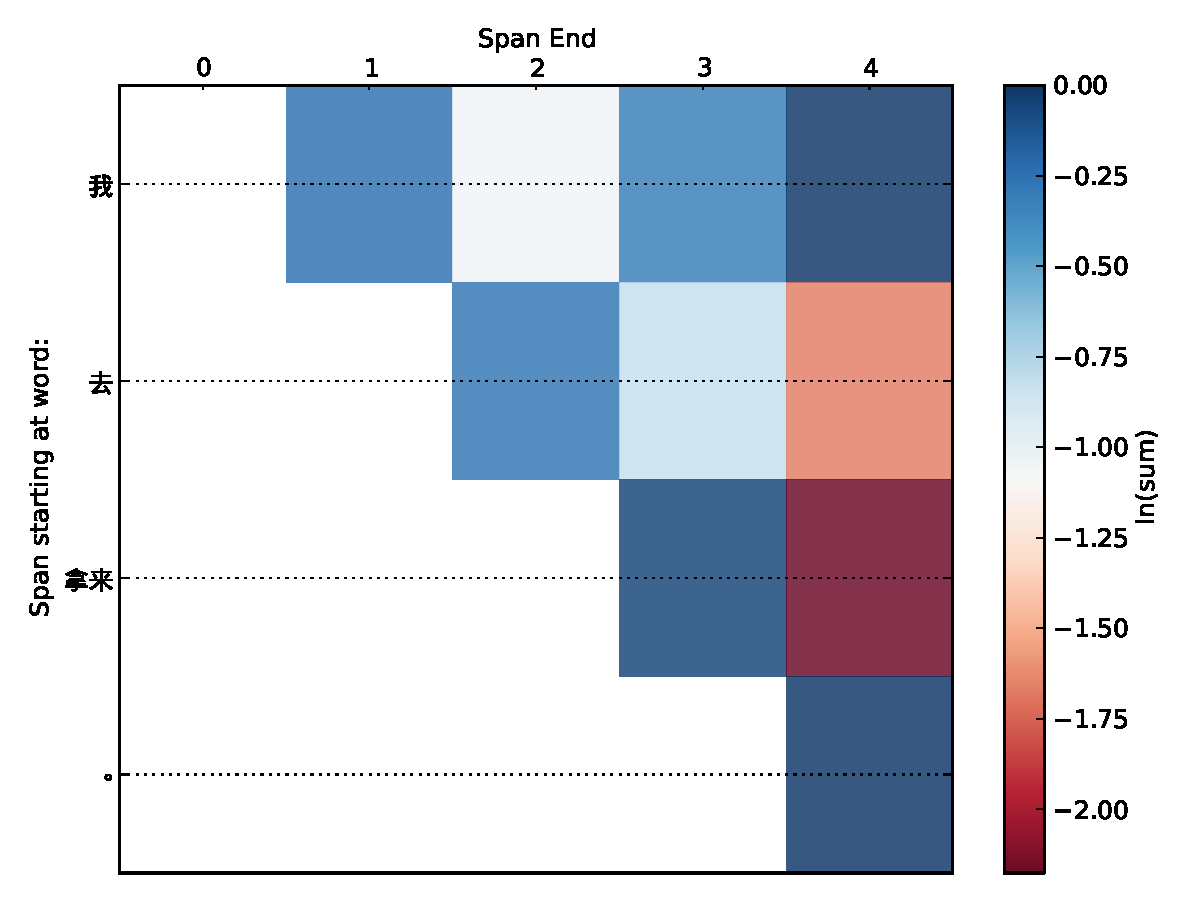
\includegraphics[width=1.1\columnwidth,keepaspectratio=true]{./spec0.pdf}		
		I 'll bring it .
		\caption {\small Spectral $m=16$ RI}
		\label{fig:spec0}
	\end{subfigure}
	\begin{subfigure}{0.67\columnwidth}
		\centering
		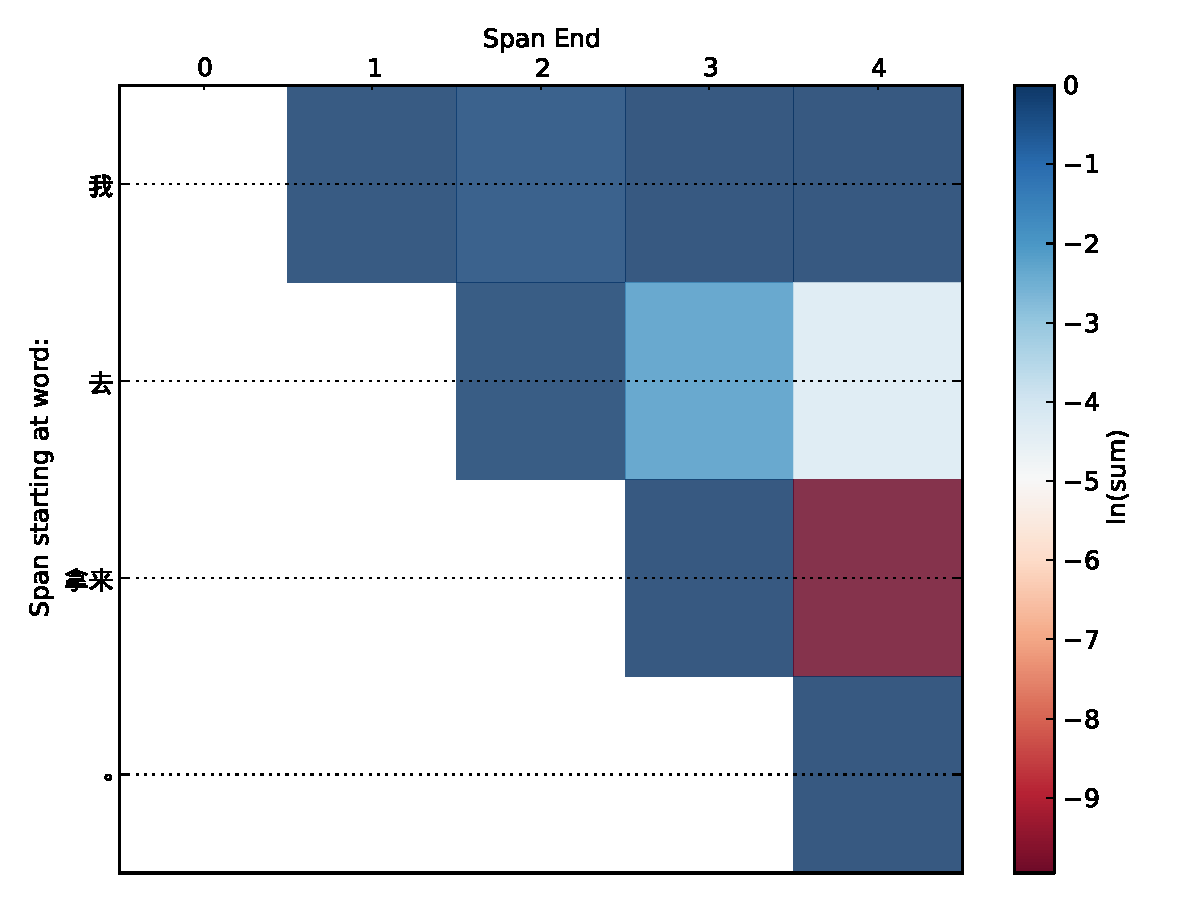
\includegraphics[width=1.1\columnwidth,keepaspectratio=true]{./em0.pdf}		
		I 'll bring it .
		\caption {\small EM $m=16$}
		\label{fig:em0}
	\end{subfigure}
	\end{center}
	\begin{center}
	\begin{subfigure}{0.67\columnwidth}
		\centering
		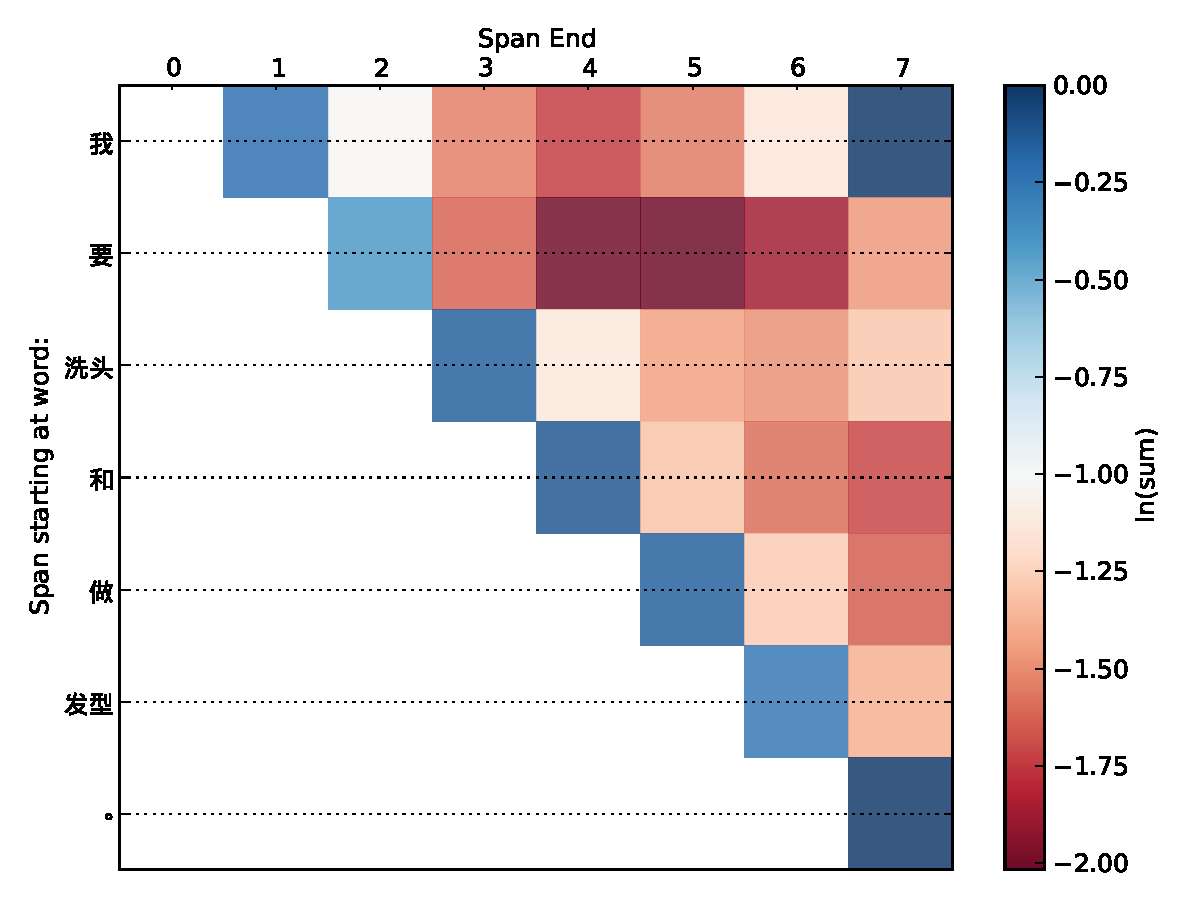
\includegraphics[width=1.1\columnwidth,keepaspectratio=true]{./mle1.pdf}	
		I 'd like a shampoo and style .
		\caption{\small MLE}
		\label{fig:mle1}			
	\end{subfigure}
	\begin{subfigure}{0.67\columnwidth}
		\centering
		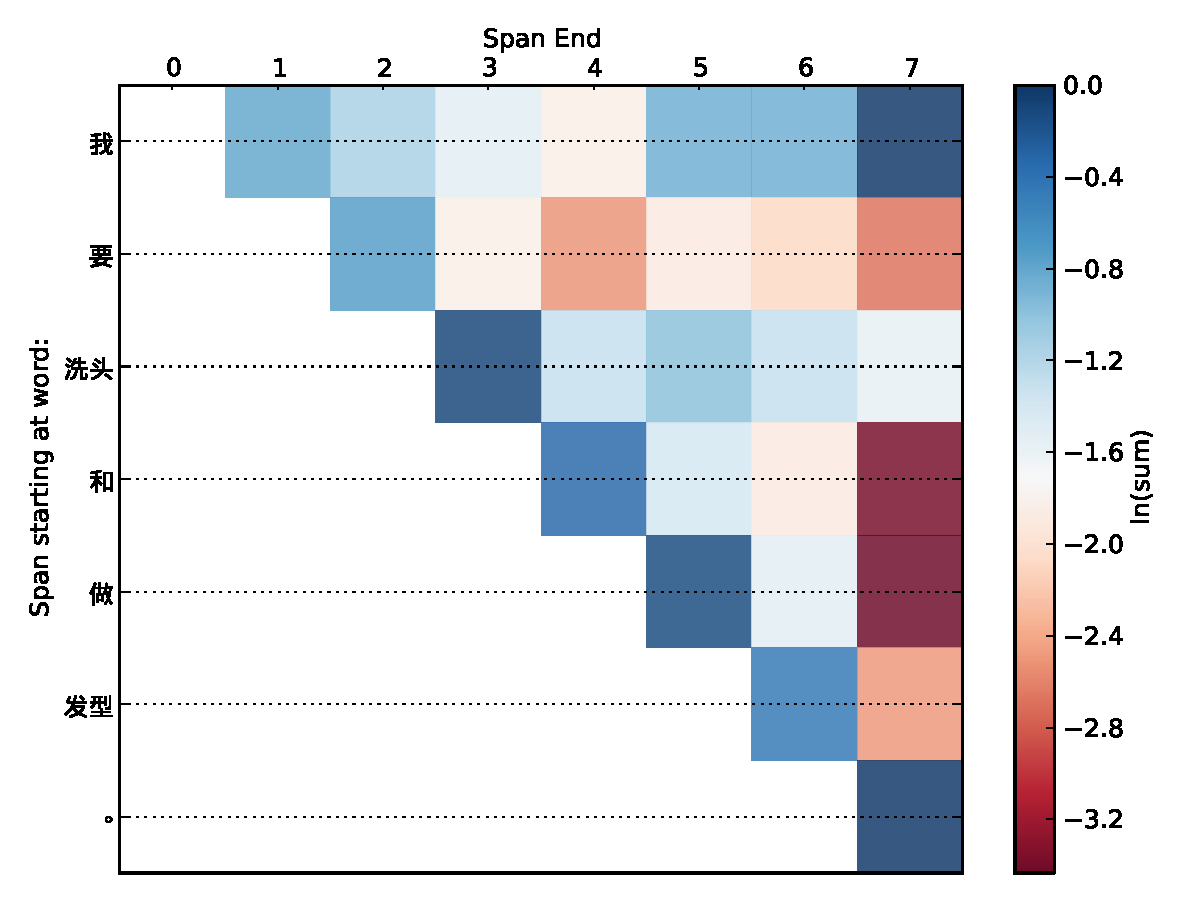
\includegraphics[width=1.1\columnwidth,keepaspectratio=true]{./spec1.pdf}		
		I 'd like a shampoo and style .
		\caption {\small Spectral $m=16$ RI}
		\label{fig:spec1}
	\end{subfigure}
	\begin{subfigure}{0.67\columnwidth}
		\centering
		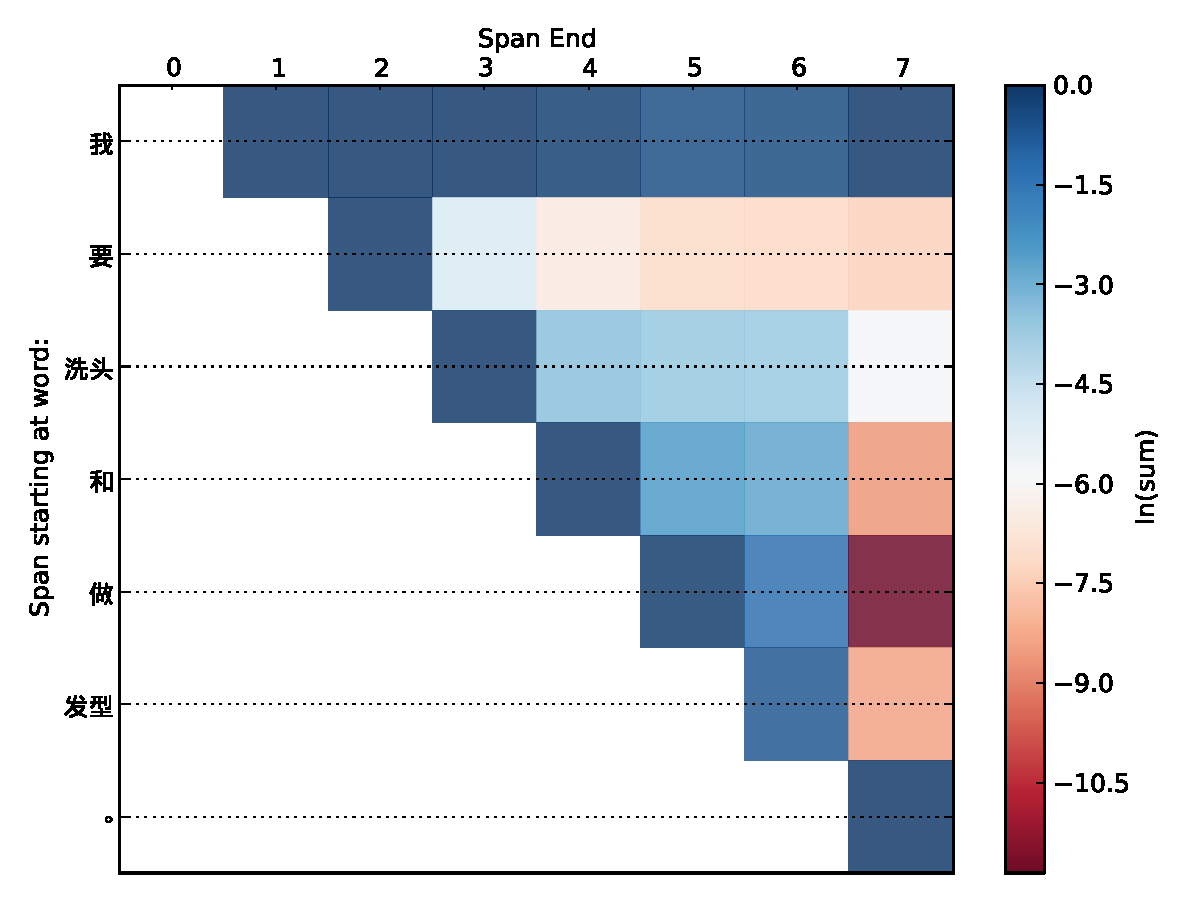
\includegraphics[width=1.1\columnwidth,keepaspectratio=true]{./em1.pdf}		
		I 'd like a shampoo and style .
		\caption {\small EM $m=16$}
		\label{fig:em1}
	\end{subfigure}
	\end{center}	
	\caption{\small A comparison of the CKY charts containing marginal probabilities of non-terminal spans $\mu(\bX, i, j)$ for the MLE, spectral $m=16$ with rule indicator features, and EM $m=16$, for the two Chinese sentences.  
	Higher likelihoods are in blue, lower likelihoods in red. 
	The hypotheses produced by each setup are below the heat maps.}
	\label{fig:heatmaps}
\end{figure*}

Figure \ref{fig:heatmaps} presents a comparison of the non-terminal span marginals for two sentences in the development set.  
We visualize these differences through a heat map of the CKY parse chart, where the starting word of the span is on the rows, and the span end index is on the columns.  
Each cell is shaded to represent the marginal of that particular non-terminal span, with higher likelihoods in blue and lower likelihoods in red. 

For the most part, marginals at the leaves (i.e., preterminal marginals) tend to score relatively similarly across different setups. 
Higher up in the chart, the latent SCFG marginals look quite different than the MLE parameters.  
Most noticeably, spans starting at the beginning of the sentence are much more favored. 
It is these rules that allow the right translation to be preferred since the MLE chooses not to place the object of the sentence in the subject's span.  
However, the spectral parameters seem to discriminate between these higher-level rules better than EM, which scores spans starting with the first word uniformly highly.  
Another interesting point is that the range of likelihoods is much larger in the EM case compared to the MLE and spectral variants. 
For the second sentence (row), the hypotheses produced by all systems are the same, but the heat map accentuates the previous observation. 

\section{Related Work}
\label{sec:related}
The goal of refining single-category HPBT grammars or automatically learning the NT categories in a grammar, instead of relying on noisy parser outputs, has been explored from several different angles in the MT literature. 
\newcite{Blunsom2008} present a Bayesian model for synchronous grammar induction, and place an appropriate nonparametric prior on the parameters. 
However, their starting point is to estimate a synchronous grammar with multiple categories from parallel data (using the word alignments as a prior), while we aim to refine a fixed grammar with additional latent states.  
Furthermore, their estimation procedure is extremely expensive and is restricted to learning up to five NT categories, via a series of mean-field approximations. 

Another approach is to explicitly attach a real-valued vector to each NT: \newcite{Huang2010} use an external source-language parser for this purpose and score rules based on the similarity between a source sentence parse and the information contained in this vector, which explicitly requires the integration of a good-quality source-language parser. 
The EM-based algorithm that we propose here is similar to what they propose, except that we need to handle tensor structures.  
\newcite{Mylonakis2011} select among linguistically motivated nonterminal labels with a cross-validated version of EM. Although they consider a restricted hypothesis space, they do marginalize over different derivations therefore their inside-outside algorithm is $\mathcal{O}(n^6)$.  

The idea of automatically learned grammar refinements comes from the monolingual parsing literature, where phenomena like head lexicalization can be modeled through latent variables.  \newcite{Matsuzaki2005} look at a likelihood-based method to split the NT categories of a grammar into a fixed number of sub-categories, while \newcite{Petrov2006} learn a variable number of sub-categories per NT.  The latter's extension is not particularly applicable to single-category grammars, but may be useful for finding the optimal number of latent states from the data.  

\newcite{Hsu2009} presented one of the initial efforts at spectral-based parameter estimation (using SVD) of observed moments for latent variable models, in the case of Hidden Markov models. 
This idea was extended to L-PCFGs \cite{cohen-14b}, and our approach can be seen as a bilingual or synchronous generalization, particularly the tensor formulation.  
We base our parameter estimation algorithm on the follow-up work of \newcite{Cohen2013}.  
%Other latent variable models like latent Dirichlet allocation \cite{Blei2003} have also been tackled spectrally \cite{Anandkumar2012}.  

The question of whether we can incorporate additional contextual information in minimal rule grammars in MT via auxiliary models instead of using longer, composed rules has been investigated before as well.
$n$-gram translation models \cite{Marino2006,Durrani2011} seek to model long-distance dependencies and reorderings through $n$-grams.  
Similarly, \newcite{Vaswani2011} use a Markov model in the context of tree-to-string translation, where the parameters are Kneser-Ney smoothed \cite{Kneser1993}, while in our instance we capture this smoothing effect through low rank or latent states.    
\newcite{Feng2013} also utilize a Markov model for MT, but learn the parameters through a more sophisticated estimation technique that makes use of Pitman-Yor hierarchical priors. 

\section{Conclusion}
In this work, we presented an approach to refine synchronous grammars used in MT by inferring the latent categories for the single nonterminal in our grammar rules, and proposed two algorithms to estimate parameters for our latent variable model.  
By fixing the synchronous derivations of each parallel sentence in the training data, it is possible to avoid many of the computation issues associated with synchronous grammar induction. 
Improvements over a minimal grammar baseline and equivalent performance to a hierarchical phrase-based baseline are achieved by the spectral approach.   
For future work, we will seek to relax this consideration and jointly reason about nonterminal categories and derivation structures.

% include your own bib file like this:
\bibliographystyle{acl}
\bibliography{bibliography}

\end{document}
